% Definition der Klasse des Dokumentes
\documentclass[11pt, a4paper]{article}

\usepackage[T1]{fontenc}        % Sorgt u.a. dafür, dass Texte vernünftig markierbar werden auch bei Sonderzeichen
\usepackage{ae,aecompl} %bessere Schrift
\usepackage{gensymb}
\usepackage[ngerman]{babel}     % Deutsches Wörterbuch usw.
\usepackage{epstopdf}   % Wandelt .eps Dateien automatisch um
\usepackage{url}    % für URL mit \url{.....}
\usepackage[font=small,labelfont=bf]{caption}       % Optionen für Bild- und Codeunterschriften
\usepackage[hidelinks]{hyperref}                    % damit Links in der PDF anklickbar werden
\usepackage{booktabs}   % bessere Tabellen mit Abstand zur hline
\pagenumbering{arabic}
\usepackage[babel,german=guillemets]{csquotes} %deutsches Anführungszeichen
\usepackage{float} %bessere Positionierungsoptionen

% Standardpakete für deutsche Sprache
\usepackage[utf8]{inputenc}
\usepackage[ngerman]{babel}

% Volle Seite nutzen
\usepackage{fullpage} 
\headsep 1cm
\parindent 0cm

% einige Pakete für Mathematische Darstellung
\usepackage{amssymb, amstext, amsmath}
\usepackage{fancyhdr}

% ein Paket für die Zählung von Seiten
\usepackage{count1to}
\usepackage{lastpage} 

%Paket für Aufzählungsbuchstaben
\usepackage{enumitem}

\usepackage{nameref}


% HIER DIE NAMEN UND EMAIL ANPASSEN
\def \ATutantName{Moritz Breipohl}
\def \ATutantEmail{mbreipohl@techfak.uni-bielefeld.de}
\def \BTutantName{Markus Rothgänger}
\def \BTutantEmail{mrothgaenger@techfak.uni-bielefeld.de}
% HIER DIE VERSUCHSNUMMER ANPASSEN
\def \Versuchsnummer{Versuch 6}
% HIER DIE GRUPPENNUMMER ANPASSEN
\def \Gruppennummer{Gruppe 5}
% HIER DEN TUTORNAMEN ANPASSEN
\def \Tutorname{Lukas Schmidt, Robin Ewers}

% Kopfzeile und Fußzeile
\lhead{\Versuchsnummer}
\chead{\textbf{Digitalelektronisches Praktikum}}
\rhead{\today}
\lfoot{\Gruppennummer}
\rfoot{\thepage\ von \pageref{LastPage}}
\cfoot{}

% Wird zur Einbindung von Bildern benötigt
\usepackage{graphicx}
\graphicspath{{images/}}

% Physikalische Einheiten darstellen
\usepackage{siunitx}

% Einbinden des Literaturverzeichnisses
\usepackage[style=numeric-comp]{biblatex}
\bibliography{literatur.bib}

% Wird zum Einbinden von LaTeX Code benötigt
\usepackage{color}
\usepackage{showexpl}
\lstset
{
    language=[LaTeX]TeX,
    breaklines=true,
    basicstyle=\tt\scriptsize,
    keywordstyle=\color{blue},
    identifierstyle=\color{magenta},
}

\renewcommand{\footrulewidth}{0.4pt}
\pagestyle{fancy}

% Konfiguration des Deckblatts
\begin{titlepage}
\title{\textbf{Digitalelektronisches Praktikum\\ Versuch 6}}
\author{\ATutantName \\ \emph{\ATutantEmail} \and \BTutantName\\ \emph{\BTutantEmail}}
\date{\Gruppennummer \\[3ex] Tutor: \Tutorname \\[3ex] \today}
\end{titlepage}

\begin{document}
% Einfügen des Deckblatts
\clearpage
\maketitle
\thispagestyle{empty}
\newpage

%%%%%%%%%%%%%%%%%%%%%%%%%%%%%%%%%%%%%%%%%
%%% Ab hier Beginn des Laborberichts: %%%%%%%%%%%%%%%%%%%%%
\section*{Theorie/Allgemeines}
- Was ist ein FPGA?
- Schritte von graphischem Aufbau zu Bitsream / Schaltung
\section*{Versuchsaufbau}
Die allgemeine Benutzung der Software Vivado wird hier nicht erläutert.
\subsection*{Aufgabe}
Es wurden insgesamt sechs Aufgaben bearbeitet. Alle arbeiteten mit den Komponenten auf dem Board.
\begin{itemize}
	\item 1. In der ersten Aufgabe sollten sechs Segmente einer Sieben-Segment-Anzeige mit Hilfe von Vier Schaltern angesteuert werden.
	Dabei sollte der angezeigte Wert der Anzeige dem Binär kodierten Wert der Schalter entsprechen. Der Block zum Ansteuern der Sechs Segmente war vorgegeben. Die Funktionalität der Implementierung sollte (durch die Simulation mit der \textit{Testbench} und auf dem Board) verifiziert und die Aufgabe der \textit{Testbench} erklärt werden. Des weiteren sollte herausgearbeitet werden, welches Segment nicht angesteuert wird, sowie, welche Aufgabe das Ausgangssignal mit dem Code \textit{AN} besitzt.
	\item 2. Im zweiten Teil war die Schaltung aus der ersten Aufgabe so zu erweitern, so dass auch das siebte Segment angesteuert wird. Dazu sollte eine aufgestellte Schaltlogik mithilfe des Karnaugh-Plans minimiert werden. Diese minimierte Schaltung wurde in das Block Design eingebaut. Auch dieses Block Design wurde durch die Simulation sowie am Board verifiziert.
	\item 3. Hier wurde das Erstellen eines \textit{IP-Core} (aus Zeitmangel) übersprungen. Es war herauszustellen, was bei dem Ansteuern aller vier Sieben-Segment-Anzeigen zu beachten ist. Diese Schaltung war zu skizzieren, zu implementieren und zu testen.
	\item 4. In der vierten Aufgabe sollten die mit den Schaltern eingestellten Werte erst bei einem Knopfdruck auf die Anzeige übernommen werden. Dazu waren alle möglichen Einbaustellen für Speicherelemente aufzuzählen und gegeneinander abzuwägen.
	Die Schaltung war zu implementieren und zu testen.
	\item 5. Im fünften Teil war das Zurücksetzen der Anzeige auf den Wert \textit{0000} bei Knopfdruck (eines weiteren Knopfes) zu implementieren. Es sollte erklärt werden, wieso sowohl der Knopf zum Zurücksetzen, als auch der Knopf zum Speichern zu drücken war, um die Anzeige zurückzusetzen.
	Eine Lösung dieses Problems war zu finden.
	\textit{\item 6. übersprungen}
	\item 7. Ein 16-Bit Zähler sollte erstellt werden, welcher bei einem Knopfdruck auf Null gesetzt werden konnte. Die Schaltung war zuerst mit zwei 8-Bit Addern zu skizzieren, dann zu realisieren und schließlich zu testen.
\end{itemize}
\subsection*{Aufbau und Erläuterung}
\subsection*{Verwendete Bauteile}
Basys 3 FPGA-Board, USB-Kabel, Computer mit Vivado Software.
\subsubsection*{Block Design Bauteile}
Allgemein sind alle Eingänge linksbündig und alle Ausgänge rechtsbündig.
Hier eine Liste der Bauteile mit einer kurzen Erklärung der Funktionsweise
\begin{itemize}	
	\item \textit{Constant:} Konstanter Wert, dessen Bitweite eingestellt werden kann.
	\item \textit{Slice:} Herausschneiden von bestimmten Bits des Eingangsbitstroms.
	\item \textit{Concat:} Hintereinanderfügen von zwei Bitströmen variabler Breite zu einem einzigen Bitstrom, dessen Breite der Summe der Breiten der Eingangsbitströme entspricht.
	\item \textit{and\_4:} AND-Gatter mit vier Eingängen.
	\item \textit{and\_3:} AND-Gatter mit drei Eingängen.
	\item \textit{or\_3:} OR-Gatter mit drei Eingängen.
	\item \textit{Utility Vector Logic:} Mehrzweck-Baustein; wurde in den Designs nur als Negator benutzt.
\end{itemize}

\newpage
\subsection*{Sechs-Segment-Anzeige}
\begin{figure}[htb]    
    \centering
    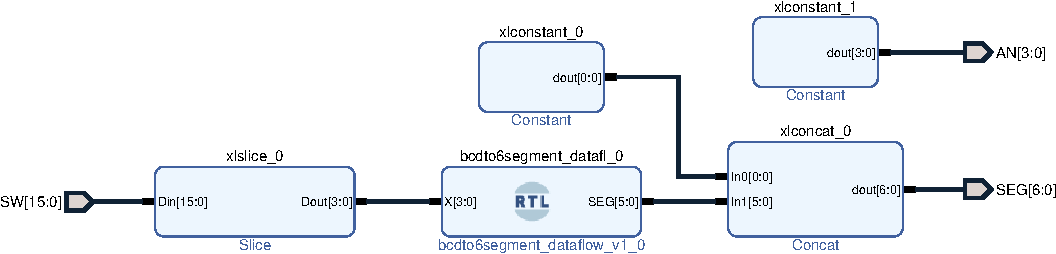
\includegraphics[width=\linewidth]{versuch1Data/seven_segment_display1.pdf}
    \caption{Block Design zum Ansteuern von Sechs der Sieben Segmente einer Anzeige}
    \label{aufbauSechsSegment}        
\end{figure}
Das Blockdesign zu dem ersten Aufbau war im wesentlichen vorgegeben. Wie in \autoref{aufbauSechsSegment} zu sehen, wurde zuerst der Bitstrom aus dem Eingang der Schalter mit Hilfe des \textit{slice} Bausteins auf die unteren vier Bit verkleinert. Diese dienen dem aus den Aufgabendaten entnommenen Modul zum ansteuern der sechs Segmente als Eingang (in der Abbildung mit \textit{bcdto6segment\_dataflow} bezeichnet). Der Ausgang des Moduls wurde mit einer ein Bit Konstante mit dem Wert $0$ verknüpft und der entstehende sieben Bit breite Strom wurde an den Ausgang \textit{SEG} geleitet. Dieser steuert die Segmente direkt an.
Zusätzlich sollte eine vier Bit breite Konstante mit dem Wert $1$ an den Ausgang \textit{AN} angelegt werden. Die Bedeutung dieses Wertes wird im folgenden Erläutert.

\subsubsection*{Test und Auswertung der Waveforms}
Bei einer Simulation mit der initialen Konfiguration stieß die Testbench auf einen Fehler. Dieser besagte, dass der Wert an der Anode falsch gesetzt sei. Ein Blick in das Handbuch ( TODO : REFFEN!!!!!) des Boards klärte auf, dass die Anode den an dem Ausgang \textit{SEG} anliegenden Wert auf die Ziffern der Anzeige weitergibt, für die das Bit an der Anode Null ist. Ein Binärcode von 1110 bedeutet also, dass die letzte Ziffer aktiv ist, die anderen nicht.
Wurde der Wert der Konstante am Ausgang \textit{AN} also auf 14 (Wert des Binärcodes 1110) gesetzt, so lief der Test ohne Fehler.
Hieraus wird deutlich, dass die Testbench die Funktionsweise und die Vorraussetzungen für eine spezifische Schaltung verifiziert, ähnlich zu einem Unit-Test.
\begin{figure}[H]    
    \centering
    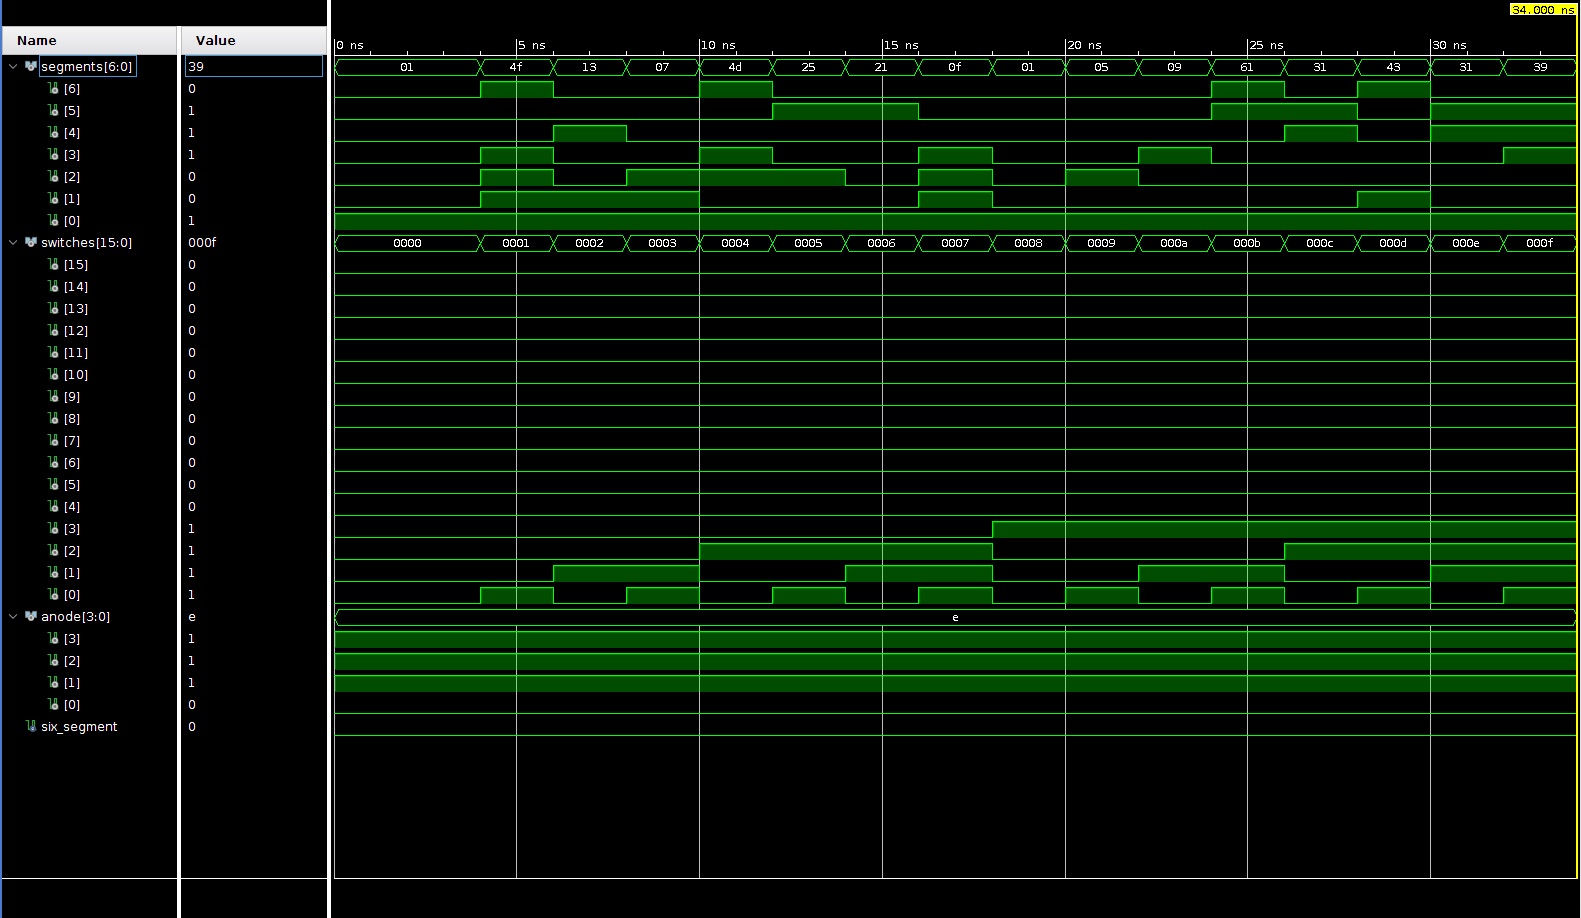
\includegraphics[width=\linewidth]{versuch1Data/waveform1.png}
    \caption{Screenshot des Waveforms der Testbench zur Sechs-Segment Anzeige}
    \label{waveformSechsSegment}        
\end{figure}
Die Waveform-Anzeige in der Software bietet die Möglichkeit, die Auswirkung von in der Testbench konfigurierten Eingangsbelegungen auf die Ausgänge zu analysieren. Somit kann das vollständige Verhalten der Schaltung verifiziert werden.
Für diesen Versuch war also in der Testbench ein Hochzählen mithilfe der letzten vier Bits des Eingangs der Schalter konfiguriert.
Konkret wurde für diesen Versuch aus den Waveforms deutlich, dass das Element, welches von dem untersten Bit des Ausgangs angesteuert wird, nicht geschaltet wird. Dieses Bit hat immer den Wert 1 (durch die Konstante im Block Design), somit leuchtet die Anzeige nicht. In dem praktischen Test wurde deutlich, dass es sich um das mittlere Segment handelt.
Beispielsweise ist in \autoref{waveformSechsSegment} zu erkennen, dass eine Null am Eingang (also der erste Abschnitt im Diagramm) in einer Ausgangsbelegung resultiert, indem alle bis auf das mittlere Element Null sind. Es wird also eine 0 als Ziffer dargestellt.

\newpage
\subsection*{Sieben-Segment-Anzeige}
Zuerst wurde eine Logiktabelle (\autoref{logikSieben}) angelegt in welcher nur das siebte Element betrachtet wurde. Alle Eingangsbelegungen der vier Eingangsbits wurden hier berücksichtigt. Ein Übertrag in einen Karnaugh-Plan (\autoref{karnaugh}) und das Erstellen einer Disjunktiven Normalform durch Umkreisen der Einsen führt zu folgender Schaltformel:
$$S_0 = \overline{x_3}\,\overline{x_2}\,\overline{x_1}\,\lor\,\overline{x_3}\,x_2\,x_1\,x_0\,\lor\,x_3\,x_2\,\overline{x_1}\,x_0$$
\begin{table}[H]
	\center
	\begin{tabular}{c|c|c|c||c}
	$x_3$ &  $x_2$ & $x_1$ & $x_0$ & Output	\\ \hline
	0 & 0 & 0 & 0 & 1 \\ \hline	
	0 & 0 & 0 & 1 & 1 \\ \hline
	0 & 0 & 1 & 0 & 0 \\ \hline
	0 & 0 & 1 & 1 & 0 \\ \hline
	0 & 1 & 0 & 0 & 0 \\ \hline
	0 & 1 & 0 & 1 & 0 \\ \hline
	0 & 1 & 1 & 0 & 0 \\ \hline
	0 & 1 & 1 & 1 & 1 \\ \hline
	1 & 0 & 0 & 0 & 0 \\ \hline	
	1 & 0 & 0 & 1 & 0 \\ \hline	
	1 & 0 & 1 & 0 & 0 \\ \hline	
	1 & 0 & 1 & 1 & 0 \\ \hline	
	1 & 1 & 0 & 0 & 1 \\ \hline	
	1 & 1 & 0 & 1 & 0 \\ \hline	
	1 & 1 & 1 & 0 & 0 \\ \hline	
	1 & 1 & 1 & 1 & 0 \\ \hline	
	\end{tabular}
	\caption{Logiktabelle zum mittleren Segment}
	\label{logikSieben}
\end{table}
\begin{table}[H]
	\center
	\begin{tabular}{c||c|c|c|c}
	$x_3 x_2 x_1 x_0$ 	& 00 & 01 & 11 & 10	\\ \hline \hline
	00 & 1 & 1 & 0 & 0 \\ \hline
	01 & 0 & 0 & 1 & 0 \\ \hline
	11 & 1 & 0 & 0 & 0 \\ \hline
	10 & 0 & 0 & 0 & 0 \\ \hline
	\end{tabular}
	\caption{Karnaugh-Plan zur Schaltung des mittleren Segments}
	\label{karnaugh}
\end{table}
Die Schaltfunktion wurde also mit AND- und OR-Gattern in das Block-Design eingefügt.
Dabei wurden zuerst die unteren vier Bits des Eingangs isoliert und negiert. Diese Bits dienten dann als Eingang für die Gatter. Schließlich wurde der Ausgang der Schaltung mit dem Ausgang des Steuerungsmoduls der sechs Segmente konkateniert.
Daraus resultierte das Design aus \autoref{aufbauSiebenSegment}.
\begin{figure}[H]    
    \centering
    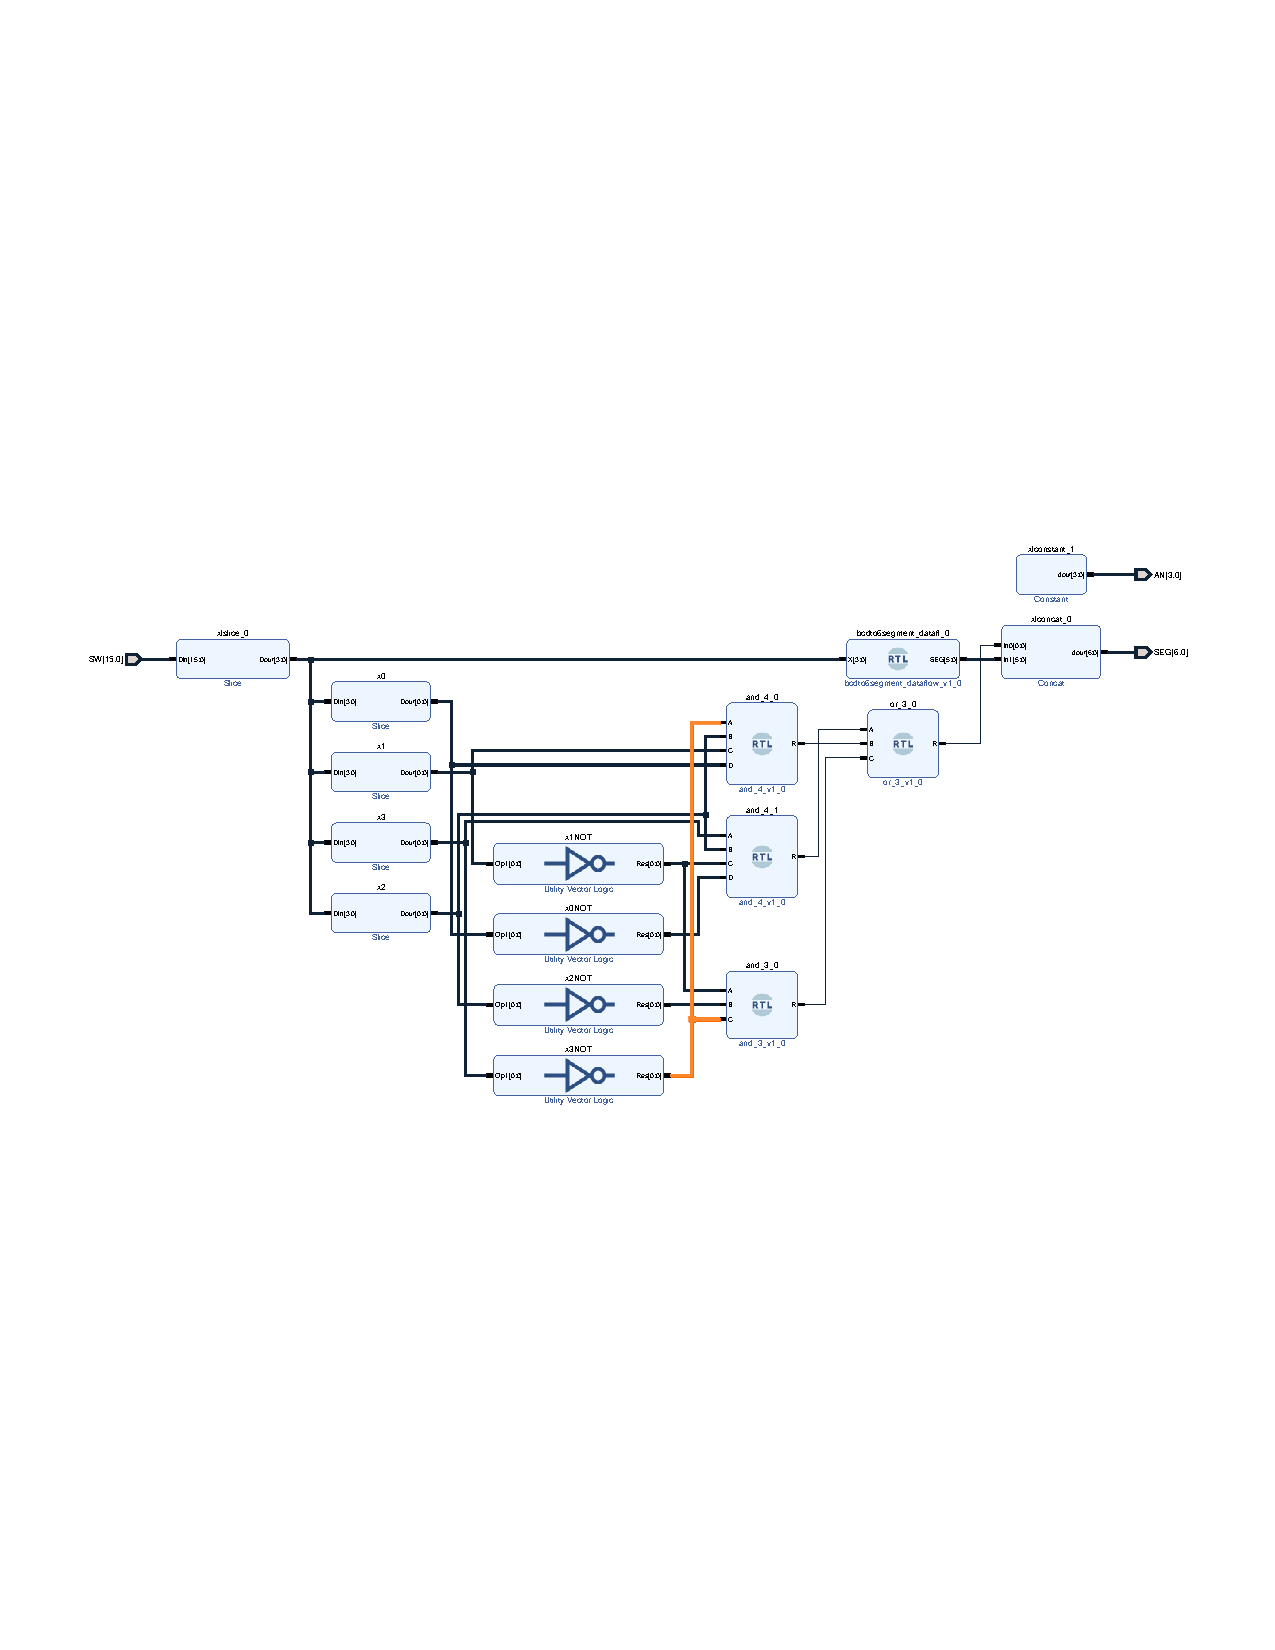
\includegraphics[width=\linewidth]{versuch2Data/seven_segment_display.pdf}
    \caption{Block Design zum Ansteuern von der vollen Sieben-Segment-Anzeige}
    \label{aufbauSiebenSegment}        
\end{figure}
\begin{figure}[H]    
    \centering
    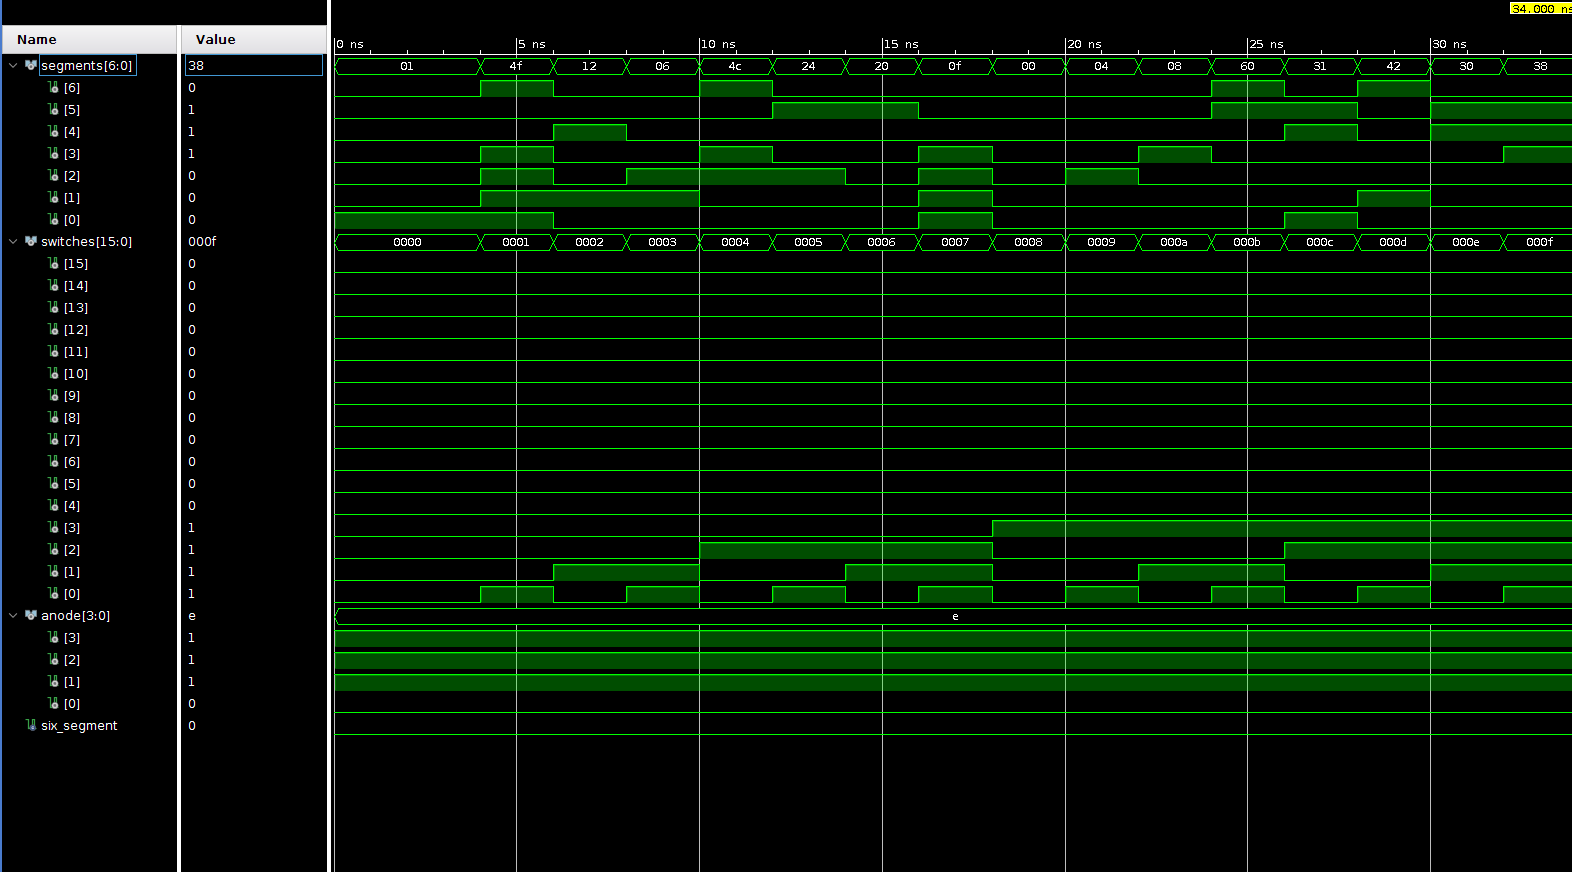
\includegraphics[width=\linewidth]{versuch2Data/aufgabe2.png}
    \caption{Screenshot des Waveforms der Testbench zur Sieben-Segment Anzeige}
    \label{waveformSiebenSegment}        
\end{figure}
Die Testbench lief ohne Fehler und die resultierenden Waveforms (\autoref{aufbauSiebenSegment}) zeigten, dass nun auch das Signal des untersten Ausgangsbit bei Variation der Eingänge verändert wurde. Ein praktischer Test lieferte das gewünschte Ergebnis.

\newpage
\subsection*{Hierarchischer Entwurf}
Problem bei einem Ansteuern von allen Ziffern auf dem Board ist, dass es nur einen Eingangskanal für alle vier Anzeigen gibt. Hier wird der Anodeneingang wichtig.

Idee war, dass jede der vier Anzeigen nacheinander zum leuchten gebracht werden.
Also wird zuerst der Wert der unteren vier Bit auf die letzte Ziffer übertragen, dann die nächsthöheren Bit auf die zweite Ziffer usw. Dies muss sehr schnell geschehen, so dass das menschliche Auge ein konstantes Leuchten wahrnimmt. Hier kommt ein Takteingang ins Spiel.

\begin{figure}[H]    
    \centering
    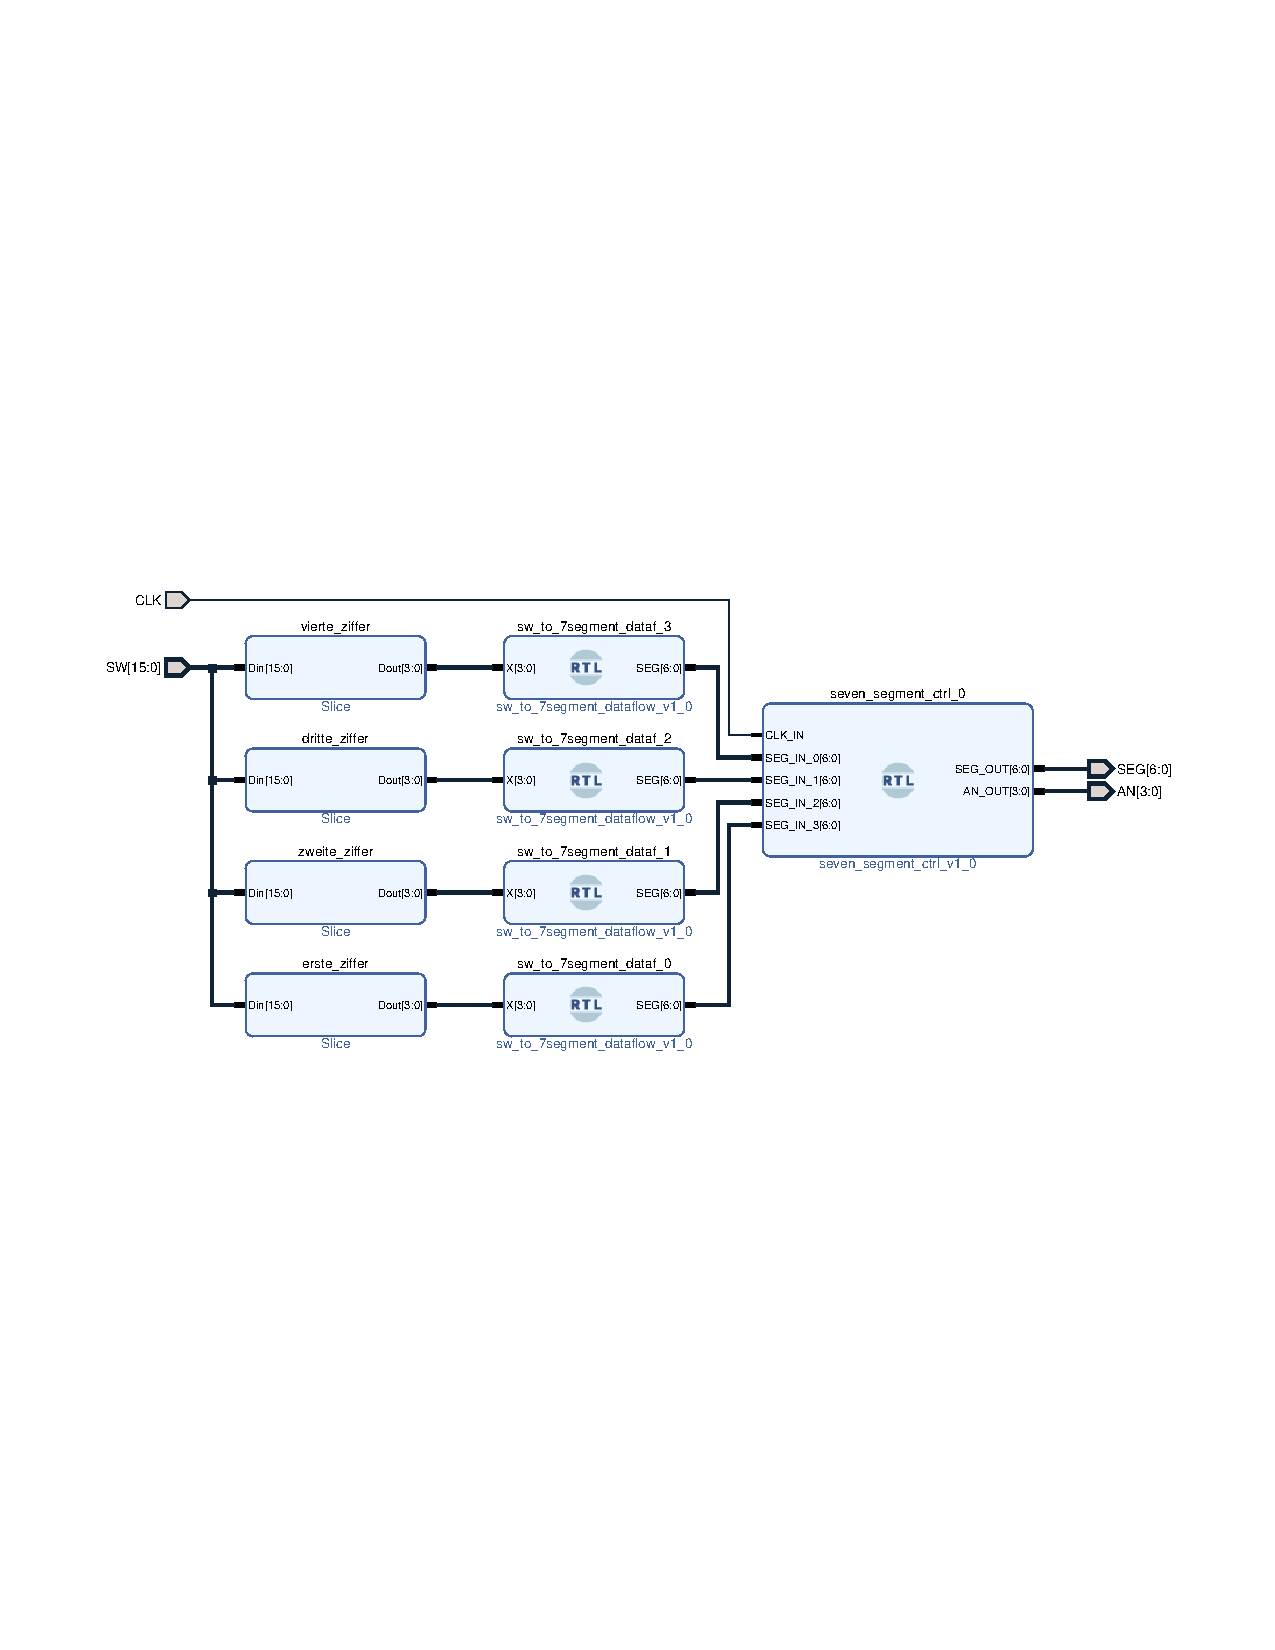
\includegraphics[width=\linewidth]{versuch3Data/hierarchical_display.pdf}
    \caption{Block Design zum Ansteuern aller vier Ziffern}
    \label{aufbauHierarchie}        
\end{figure}
\begin{figure}[H]    
    \centering
    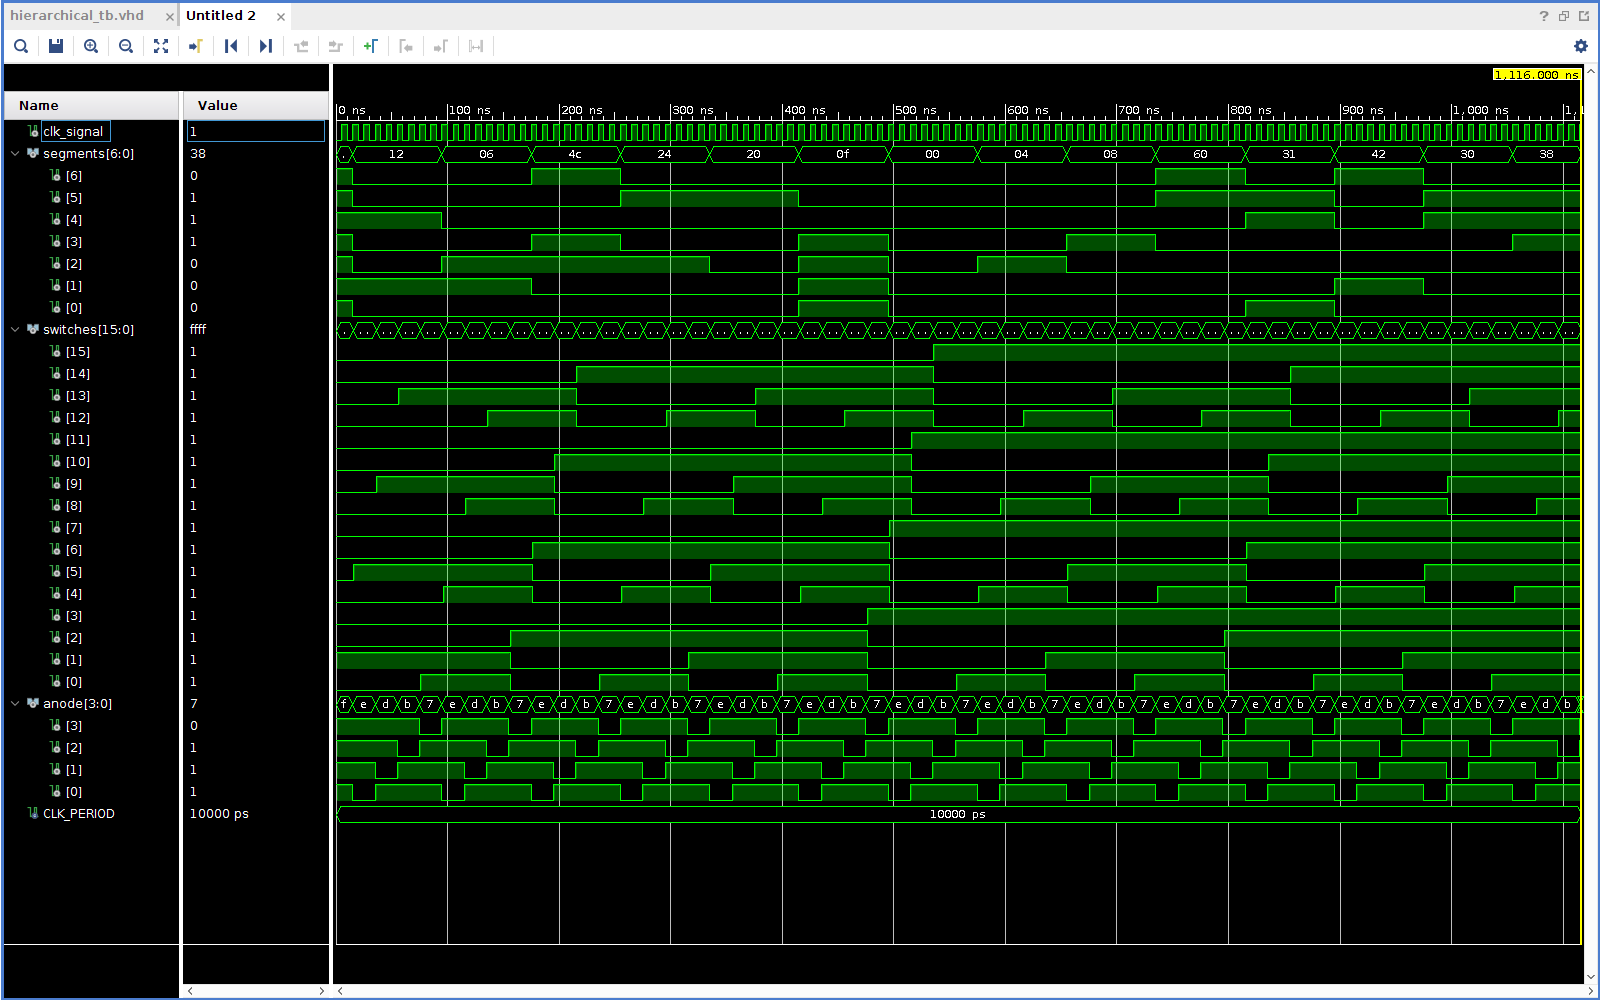
\includegraphics[width=\linewidth]{versuch3Data/hierarchical.png}
    \caption{Waveforms der Testbench beim Ansteuern aller vier Ziffern}
    \label{waveformHierarchie}        
\end{figure}

In diesem Aufbau (\autoref{aufbauHierarchie}) wurde das Modul \textit{sw\_to\_7segment\_dataf} im Design verwendet. Dieser Baustein stellt die Funktionalität aus Aufgabe 2 zur Verfügung, jedoch in einem Baustein vereinigt. Diesen Baustein selbst zu erstellen war ursprünglich Teil der Aufgabe, wurde von uns jedoch übersprungen. Es wurde also das Eingangssignal der Schalter zuerst zugeschnitten, sodass jeweils vier Bit in ein Modul zur Ansteuerung einer Anzeige geleitet wurden. Das Rotieren durch die Anode und den entsprechenden Eingang übernimmt ein ebenfalls vorgegebener Baustein mit dem Namen \textit{seven\_segment\_ctrl}. Dieser hat neben den Vier sieben Bit breiten Eingängen einen Eingang mit dem der Takt zum Umschalten bestimmt wird. Hier wurde ein neuer Eingang dem Design hinzugefügt, welcher einen Takt (Clock) mit einer Frequenz von 100 MHz erzeugte.
Die Testbench lief ohne Fehler durch (es musste eventuell der Test manuell gestartet werden, die Waveforms sind in \autoref{waveformHierarchie}) und auch das Ergebnis auf der Hardware war wie erwartet. Es war kein flackern zu sehen und mit den obersten vier Bit konnte die erste Ziffer, mit den niedrigsten vier Bit die letzte Ziffer angesteuert werden. Eine Verifizierung der Funktion war hier erstmals nicht nur anhand der Waveforms möglich. Diese zeigen nur den Ausgang zu den Segmenten sowie die Belegung der Schalter. Dennoch ist anhand der Waveforms die korrekte Belegung der Anode zu erkennen. An der Anode ist immer nur ein Bit nach dem anderen aktiv (also Null).

\newpage
\subsection*{Anzeige bei Tastendruck übernehmen}
Um diese Aufgabe zu realisieren, muss die aktuelle Belegung der Anzeige gespeichert werden. Es wurde ein beliebig breites Speicherregister (\textit{register\_gen\_bit\_enable}) mit Speicherung auf steigender Taktflanke (am \textit{Enable} Eingang) bereitgestellt. Hier gibt es mehrere Möglichkeiten zur Platzierung des Registers.
\begin{itemize}
	\item 1. Vor dem Aufteilen des Eingagnssignals. Hier ist der Vorteil, dass nur ein einziges 16-Bit Register benötigt wird.
	\item 2. Nach dem Aufteilen. Die Speicherung der Werte jeder einzelnen Ziffer ist so unabhängig möglich.
	\item 3. Nach den Logikbausteinen zum Schalten der sieben Segmente. Ähnlich zu 2., das Register ist jedoch sieben statt vier Bit breit.
\end{itemize}
Ein Speichern von Daten nach dem Controller Baustein ist nicht Sinnvoll, da der Takt das Signal ständig verändert bzw. je nach Speicherzeitpunkt die Werte einer anderen Ziffer gespeichert würden.
Am sinnvollsten erschien uns zu diesem Zeitpunkt eine Speicherung der 16-Bit Rohdaten, da die Anpassung am geringsten war. Als Eingangssignal um das Register zu aktivieren nutzten wir den Knopf auf dem Board mit der Bezeichnung \textit{BTN\_C}.
\begin{figure}[H]    
    \centering
    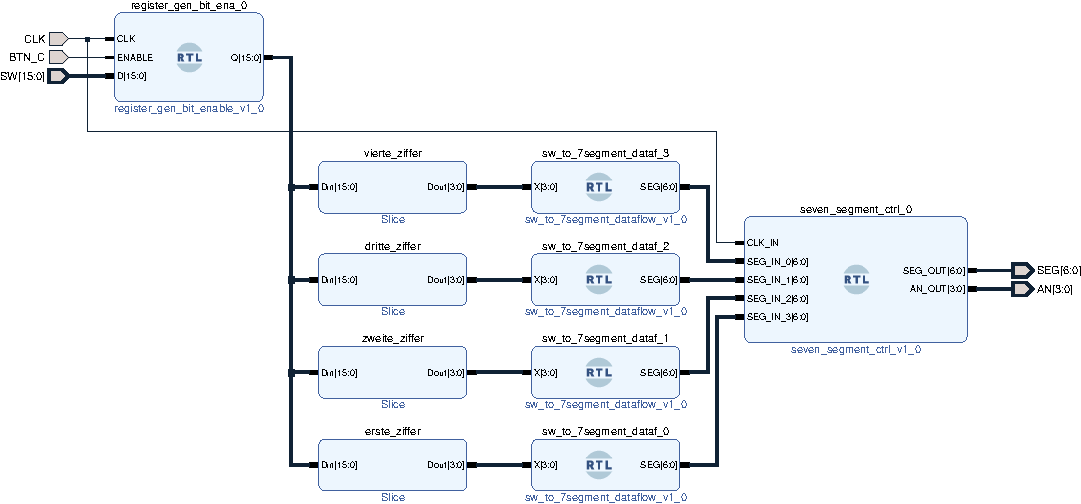
\includegraphics[width=\linewidth]{versuch4Data/hierarchical_display_trigger.pdf}
    \caption{Block Design mit Speicherregister}
    \label{aufbauTrigger}        
\end{figure}
\begin{figure}[H]    
    \centering
    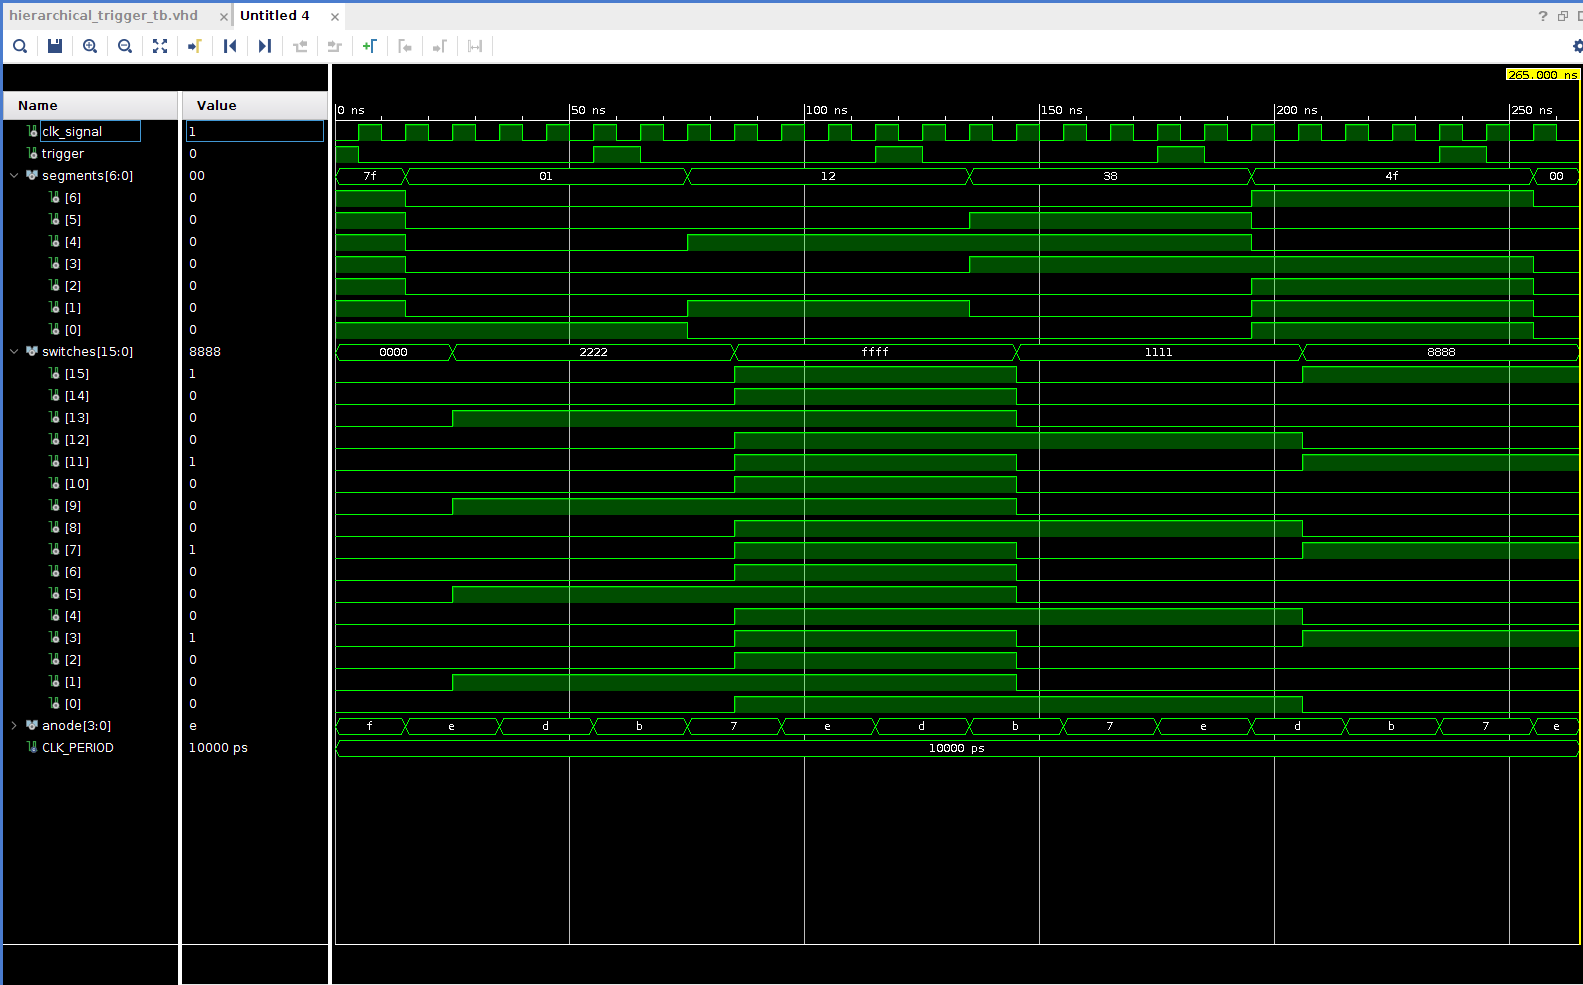
\includegraphics[width=\linewidth]{versuch4Data/hierarchical_trigger.png}
    \caption{Waveforms zur Speicherung auf Tastendruck}
    \label{waveformTrigger}        
\end{figure}
Wie im Aufbau (\autoref{aufbauTrigger}) und den Waveforms der entsprechenden Testbench (\autoref{waveformTrigger}) zu sehen, werden die an den Schaltern des Boards eingestellten Werte erst bei der nächsten Taktflanke nach drücken des Knopfes \textit{BTN\_C} (im Waveform \textit{trigger}) auf den Ausgang zu den Segmenten übernommen.

\newpage
\subsection*{Zurücksetzen der Anzeige}
Hier wurde deutlich, dass die Entscheidung, das Register an den Anfang des Datenstroms zu platzieren, für diese Aufgabe nicht optimal war. Problem war, dass uns vier Bit Multiplexer zur Verfügung standen, wir zur Lösung der Aufgabe in dieser Konfiguration allerdings zwischen zwei 16-Bit Daten wechseln müssten. Daher wurde die Schaltung so umgebaut, dass vier Vier-Bit-Register den Zustand der Anzeige nach dem Aufteilen in die vier Bitblöcke Speichern. So konnten wir dem Design pro Ziffer einen Multiplexer hinzufügen, welcher beim Drücken von \textit{BTN\_D} den Eingang des Registers mit einem vier Bit breiten Nullvektor belegte. Sobald der Knopf losgelassen wurde, wurde wieder die Belegung aus den Schaltern benutzt. 
Der Aufbau des Beschriebenen ist in \autoref{aufbauDelete} dargestellt. Die Testbench wurde ohne Fehler durchlaufen und die resultierenden Waveforms sind in \autoref{waveformDelete} zu sehen.
Um die Anzeige wirklich Zurückzusetzen, musste der Null-Wert in das Register gespeichert werden. Daher war ein gleichzeitiges Drücken von \textit{BTN\_D} (zum Wählen des Nullvektors) und \textit{BTN\_C} (zum Speichern des Nullvektors im Register) notwendig. Eine Lösung dieses Problems hätte realisiert werden können, wenn der Knopf zum Wählen des Nullvektors gleichzeitig die Register aktiviert. 
\begin{figure}[H]    
    \centering
    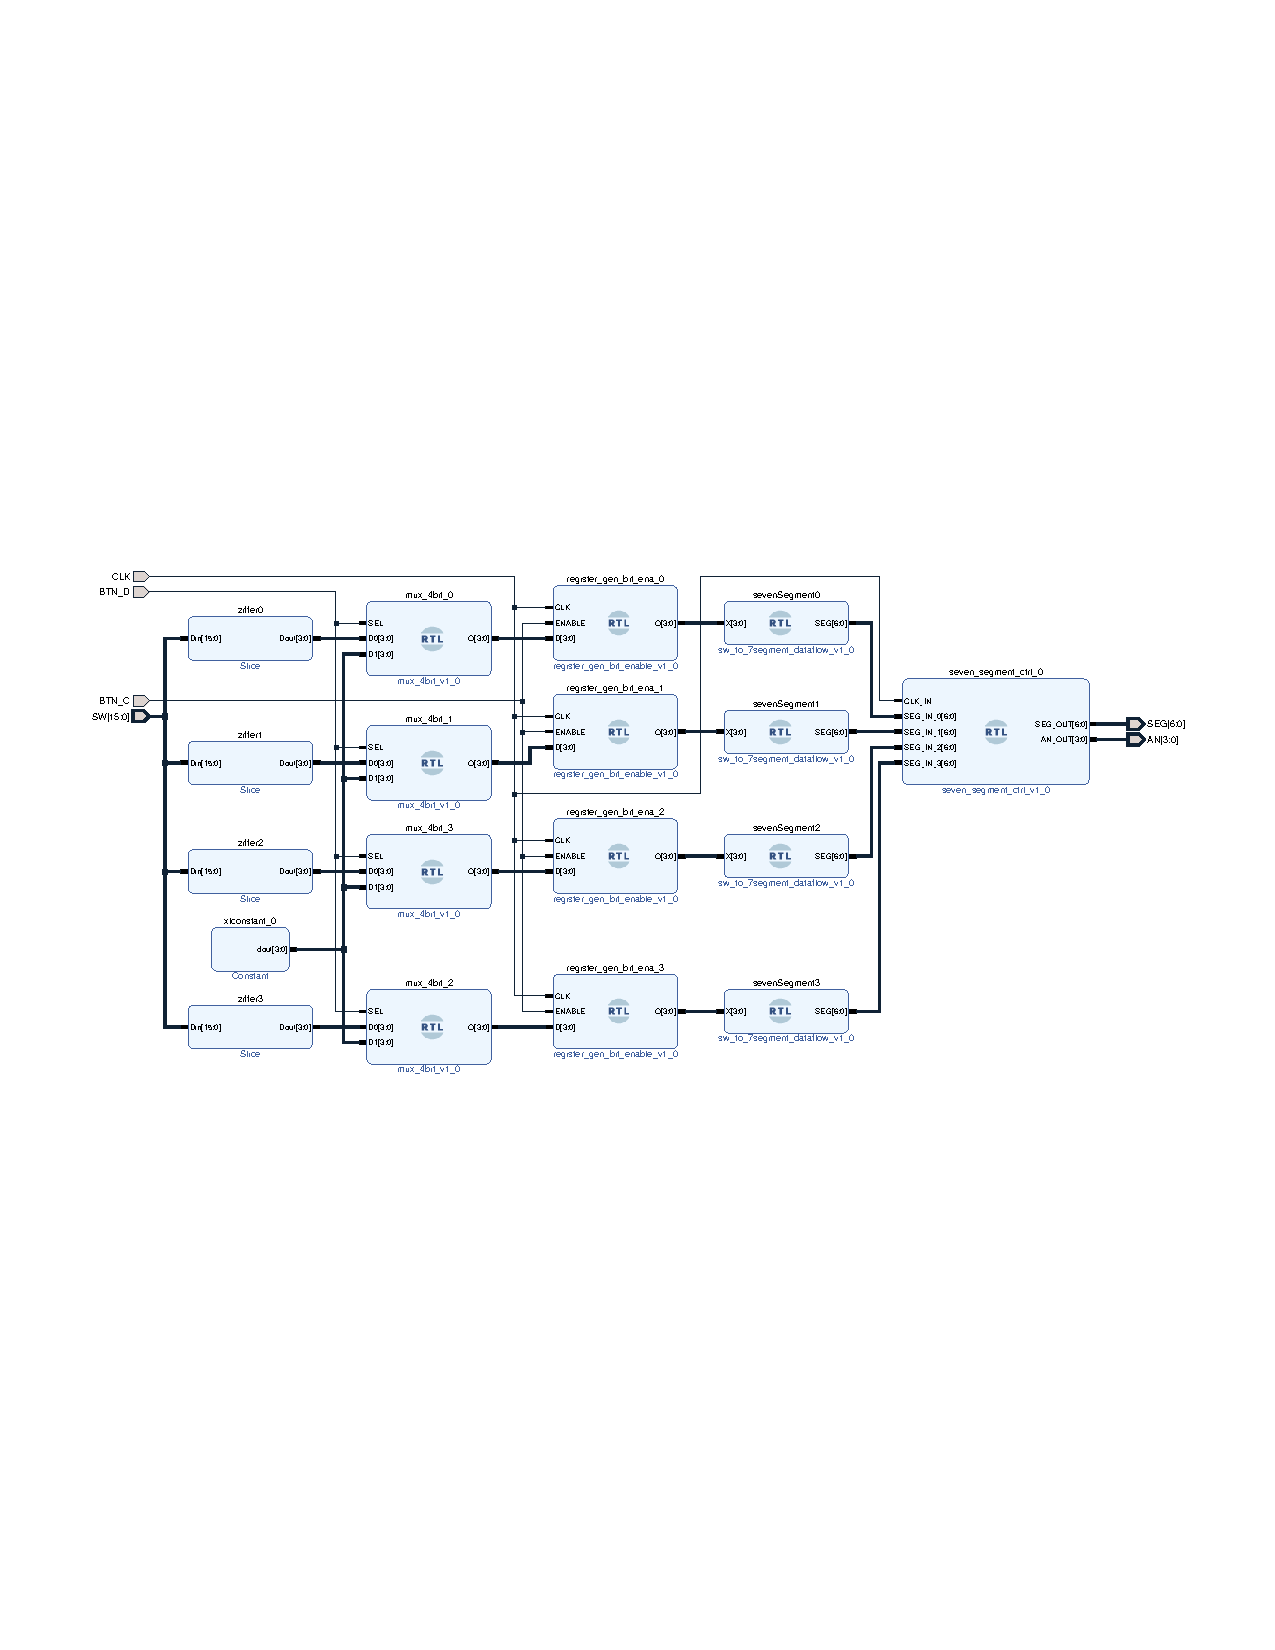
\includegraphics[width=\linewidth]{versuch5Data/hierarchical_display_delete.pdf}
    \caption{Block Design zum Zurücksetzen der Anzeige}
    \label{aufbauDelete}        
\end{figure}
\begin{figure}[H]    
    \centering
    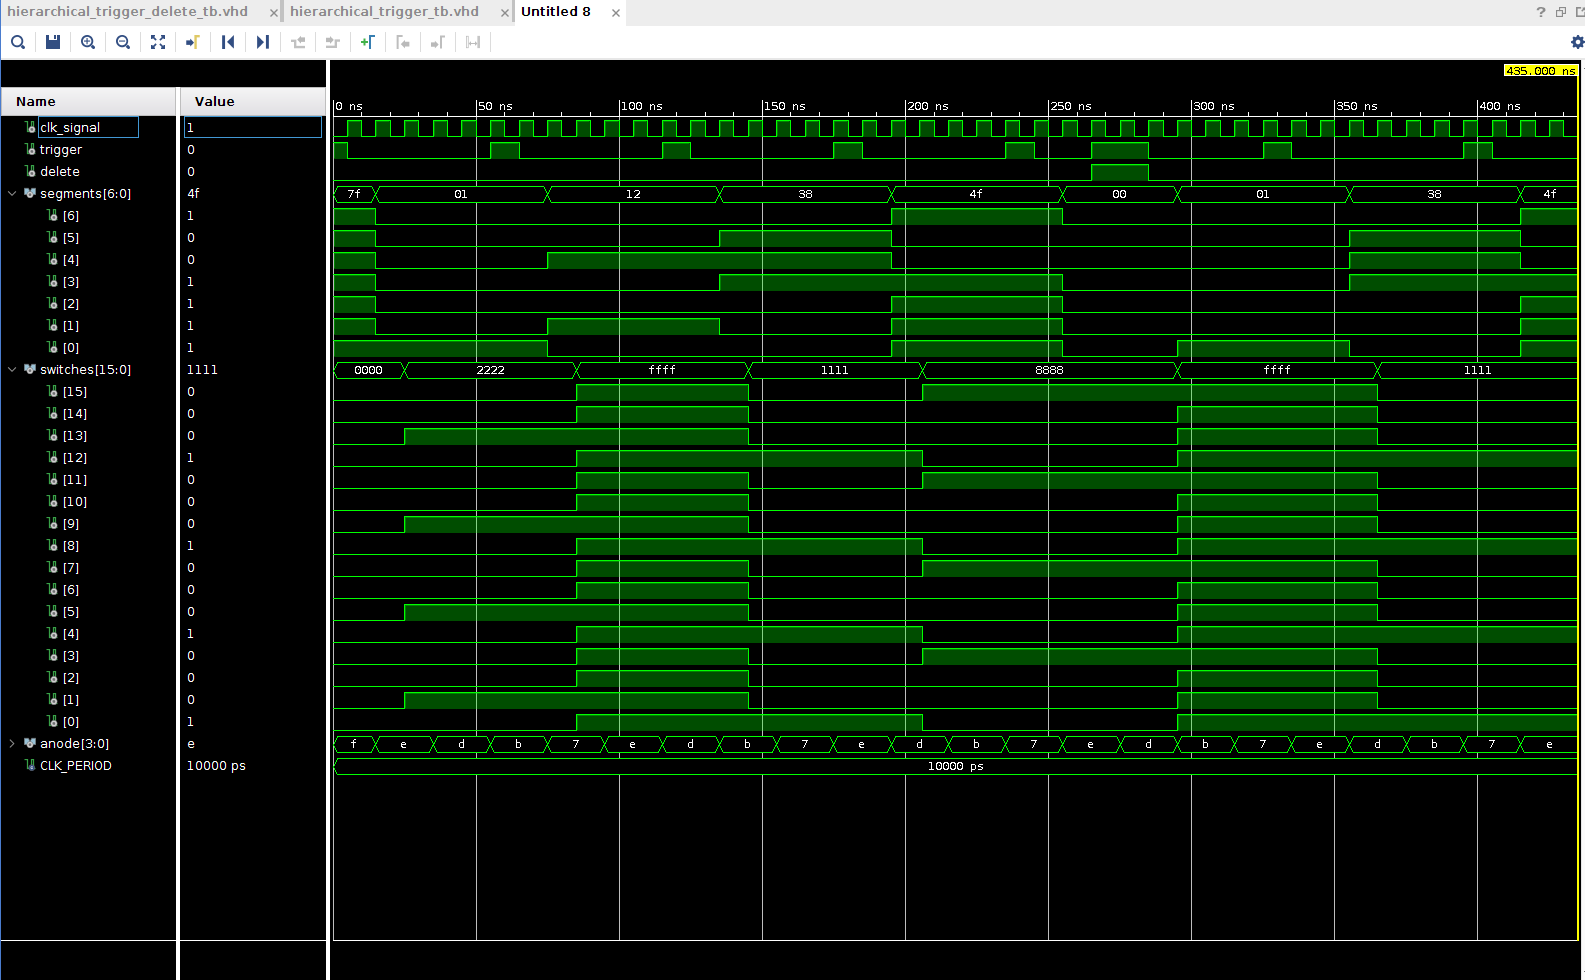
\includegraphics[width=\linewidth]{versuch5Data/hierarchicalDelete.png}
    \caption{Waveforms zum Zurücksetzen der Anzeige}
    \label{waveformDelete}        
\end{figure}

\newpage
\subsection*{16-Bit Zähler}
Um 16 Bit hochzählen zu können, wurden Addiererbausteine benötigt.
Vorgegeben waren \textit{add\_8bit\_v1\_0}, welche nur 8 Bit addieren können. 
Diese besitzen 3 Eingänge und zwei Ausgänge: zwei jeweils 8 Bit breite Inputs, die aufeinander addiert werden sollen, so wie ein Carry-Eingang, welcher 1 Bit groß ist und auf das niederwertigste Bit addiert wird; zudem einen 8 Bit breiten Output, welcher das Ergebnis der Addition bereitstellt und einen 1 Bit großen Carry-Ausgang, welcher eine 1 liefert, wenn die Addition ein Ergebnis größer als 8 Bit liefert.
\newline
Um daraus einen 16 Bit breiten Addierer zu basteln brauchten wir zwei dieser Bausteine, einer für die unteren 8 Bit und einer für die höheren 8 Bit.
Um den Überlauf der unteren 8 Bit zu zählen, wurde der Carry-Ausgang des ersten Addierers mit dem Carry-Eingang des zweiten Addierers verbunden.
Da hier in jedem Schritt eine 1 addiert werden sollte, wurde der erste Eingang des ersten Addierers eine Konstante mit 8 Bit Breite und Wert 1 verbunden.
Der andere Eingang bezog die unteren 8 Bit des Register, aufgespalten durch einen Slice-Baustein.
\newline
Für die höheren 8 Bit wurden die höherwertigen 8 Bit des Registers, wieder durch einen Splicer bezogen, sowie eine Konstante, 8 Bit breite 0 angeschlossen.
Um hier hochzählen zu können, wurde der Carry-Ausgang des anderen Addierers mit dem Carry-Eingang dieses Addierers verbunden.
Dies resultiert darin, dass wenn die niederwertigen 8-Bit ihren Speicherbereich überschreiten, die höherwertigen 8 Bit einmal hochzählen.
\newline
Die Zwischenergebnisse wurden in dem bereits bekannten Register gespeichert. Dieses hat bei einem Taktsignal auf dem Eingang \textit{CLK} den Ausgang mit den Werten am Input überschrieben. Somit liegt am Eingang des Registers immer der bereits nächste, um 1 erhöhte Wert, wird aber nur bei einem CLK-Signal durgeschaltet.
Zu beachten ist, dass das Taktsignal an dem Register durch den vorgegebenen \textit{frequency\_divider\_v1\_0} reduziert wurde, da ein Zähler, welcher mit 100 MHz hochzählt, nicht für das menschliche Auge sichtbar ist.
\newline
Hinter dem Register hängt die bereits zuvor verwendete Schaltung zum decodieren und darstellen auf dem Sieben-Segment-Display des Boards.
\newline
Zunächst hatten wir das Problem, dass unser Zähler immer 2 addierte und nicht 1. Nach etwas Suche klärte sich das Problem aber: Die Konstante \textit{xlconstant\_carry\_0} war versehentlich mit dem Wert 1 statt 0 belegt.
Nachdem das Problem behoben war, lief die Testbench einwandfrei und auch auf dem Board konnte die Schaltund verifiziert werden. Bei Druck des Knopfes \textit{BTN\_D} wurde der Zähler auf 0 zurückgesetzt.


\begin{figure}[H]    
    \centering
    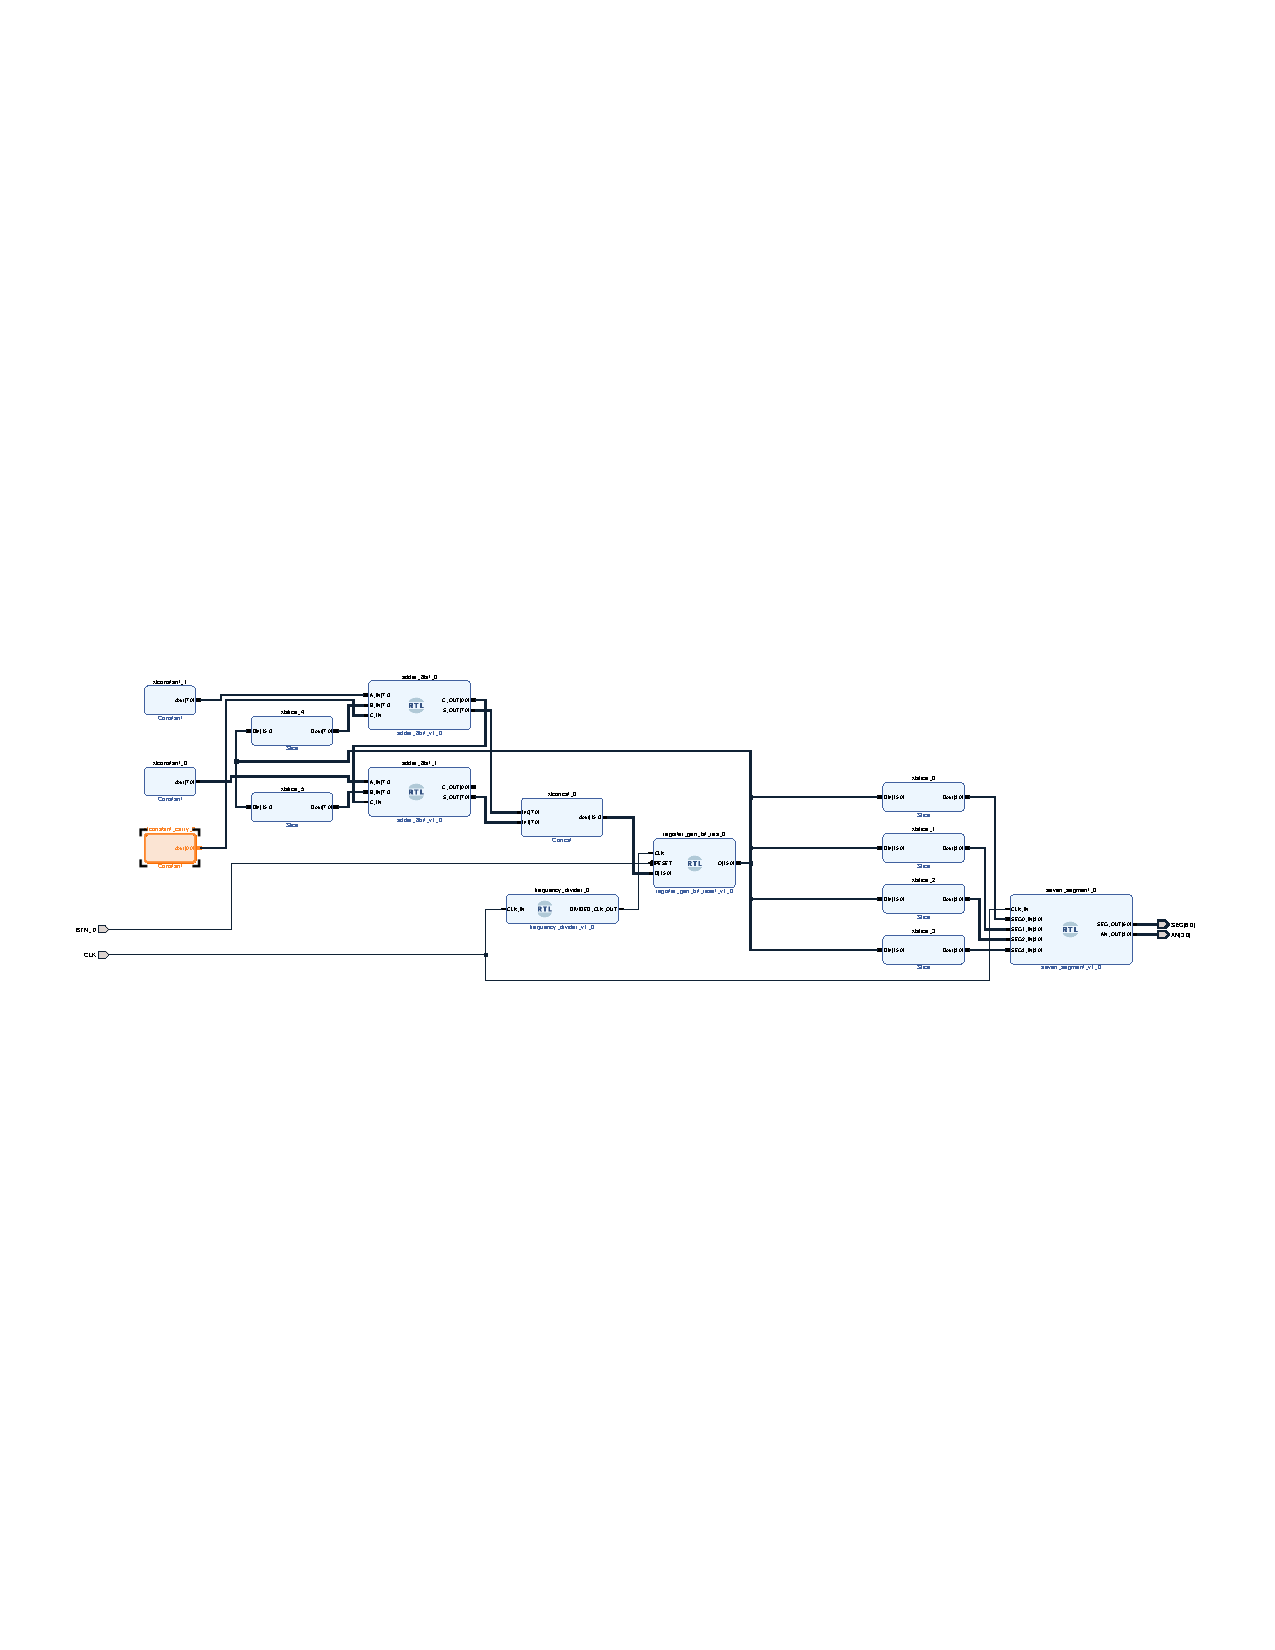
\includegraphics[width=\linewidth]{versuch7Data/counter.pdf}
    \caption{Blockdesign des 16-Bit Zählers}
    \label{aufbauZähler}        
\end{figure}
\begin{figure}[H]    
    \centering
    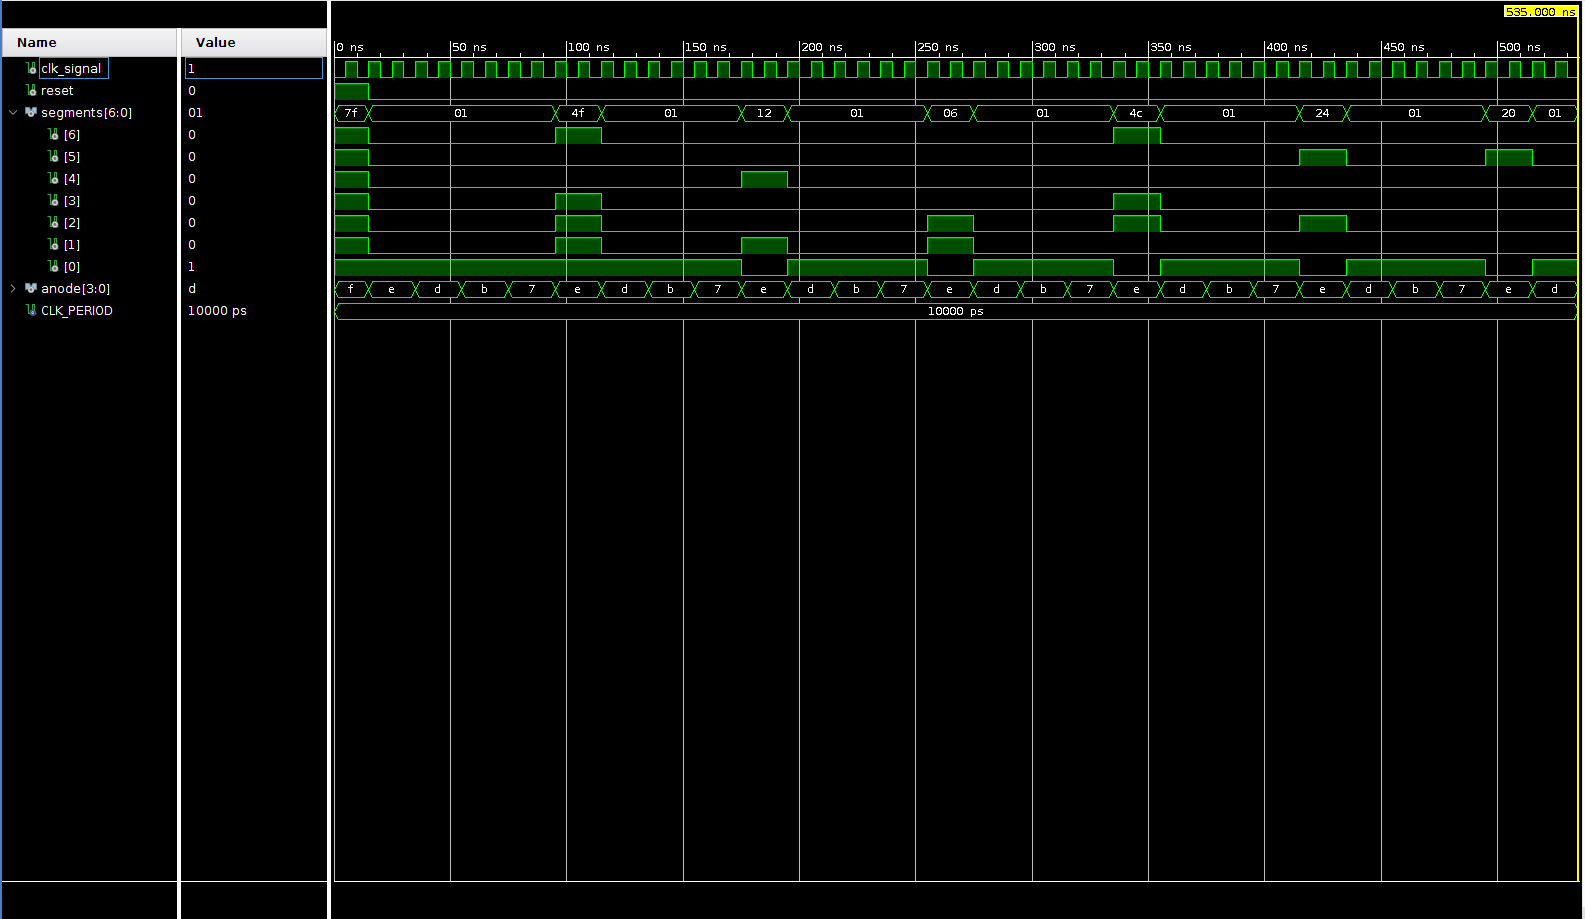
\includegraphics[width=\linewidth]{versuch7Data/counter.png}
    \caption{Waveforms zum Counter}
    \label{waveformCounter}        
\end{figure}

\section*{Fazit}
\end{document}